\documentclass{article}
\usepackage{tikz}
\usetikzlibrary{positioning, automata}
\usepackage{fancyhdr}
\usepackage{extramarks}
\usepackage[plain]{algorithm}
\usepackage{algpseudocode}
\usepackage[utf8]{inputenc} 
\usepackage[T1]{fontenc}    
\usepackage{hyperref}       
\usepackage{url}        
\usepackage{booktabs}
\usepackage{pdfpages}
\usepackage{amsfonts}   
\usepackage{nicefrac}       
\usepackage{microtype}      
\usepackage{amsmath}
\usepackage{graphicx}
\usepackage{float}
\usepackage{caption}
\usepackage{ragged2e}
\usepackage{amssymb}
\usepackage{mathtools}
\usepackage{xcolor}
\usepackage[spanish]{babel} % ¡Solo una vez!
\usepackage{array}
\usepackage{multirow}
\usepackage{multicol}
\usepackage{manfnt}
\usepackage{layout}
\usepackage{manfnt}
\usepackage{phaistos}
\usepackage{polynom}
\usepackage[inkscapeformat=png]{svg}
\usepackage[most]{tcolorbox}
\usepackage{listings}

\lstset{
    language=Python,                        % Lenguaje de programación
    basicstyle=\ttfamily\small\color[HTML]{F8F8F2}, % Fuente monoespaciada y texto blanco claro
    backgroundcolor=\color[HTML]{282A36},   % Fondo oscuro (Dracula)
    keywordstyle=\color[HTML]{FF79C6}\bfseries, % Palabras clave en rosa y negrita
    commentstyle=\color[HTML]{6272A4}\itshape, % Comentarios en gris azulado y cursiva
    stringstyle=\color[HTML]{F1FA8C},       % Cadenas en amarillo
    numberstyle=\tiny\color[HTML]{BD93F9}, % Números en lila
    identifierstyle=\color[HTML]{8BE9FD},  % Identificadores en azul claro
    emph={xlabel, ylabel, title, legend, grid}, % Destaca palabras específicas
    emphstyle=\color[HTML]{50FA7B},        % Color verde brillante para palabras destacadas
    numbers=left,                           % Números de línea a la izquierda
    stepnumber=1,                           % Mostrar número en cada línea
    numbersep=10pt,                         % Separación de los números de línea
    showstringspaces=false,                 % No marcar los espacios en las cadenas
    frame=note,                           % Marco alrededor del código
    framexleftmargin=20pt,                  % Espacio a la izquierda del marco para los números
    rulecolor=\color[HTML]{F8F8F2},         % Color del borde del marco
    breaklines=true,                        % Rompe líneas largas
    breakatwhitespace=true,                 % Rompe en los espacios
    tabsize=4,                              % Tamaño de tabuladores
    escapeinside={\%*}{*)}                  % Permite la inserción de LaTeX dentro del código
}

\lstset{literate=
  {á}{{\'a}}1 {é}{{\'e}}1 {í}{{\'i}}1 {ó}{{\'o}}1 {ú}{{\'u}}1
  {Á}{{\'A}}1 {É}{{\'E}}1 {Í}{{\'I}}1 {Ó}{{\'O}}1 {Ú}{{\'U}}1
  {à}{{\`a}}1 {è}{{\`e}}1 {ì}{{\`i}}1 {ò}{{\`o}}1 {ù}{{\`u}}1
  {À}{{\`A}}1 {È}{{\'E}}1 {Ì}{{\`I}}1 {Ò}{{\`O}}1 {Ù}{{\`U}}1
  {ä}{{\"a}}1 {ë}{{\"e}}1 {ï}{{\"i}}1 {ö}{{\"o}}1 {ü}{{\"u}}1
  {Ä}{{\"A}}1 {Ë}{{\"E}}1 {Ï}{{\"I}}1 {Ö}{{\"O}}1 {Ü}{{\"U}}1
  {â}{{\^a}}1 {ê}{{\^e}}1 {î}{{\^i}}1 {ô}{{\^o}}1 {û}{{\^u}}1
  {Â}{{\^A}}1 {Ê}{{\^E}}1 {Î}{{\^I}}1 {Ô}{{\^O}}1 {Û}{{\^U}}1
  {ã}{{\~a}}1 {ẽ}{{\~e}}1 {ĩ}{{\~i}}1 {õ}{{\~o}}1 {ũ}{{\~u}}1
  {Ã}{{\~A}}1 {Ẽ}{{\~E}}1 {Ĩ}{{\~I}}1 {Õ}{{\~O}}1 {Ũ}{{\~U}}1
  {œ}{{\oe}}1 {Œ}{{\OE}}1 {æ}{{\ae}}1 {Æ}{{\AE}}1 {ß}{{\ss}}1
  {ű}{{\H{u}}}1 {Ű}{{\H{U}}}1 {ő}{{\H{o}}}1 {Ő}{{\H{O}}}1
  {ç}{{\c c}}1 {Ç}{{\c C}}1 {ø}{{\o}}1 {å}{{\r a}}1 {Å}{{\r A}}1
  {€}{{\euro}}1 {£}{{\pounds}}1 {«}{{\guillemotleft}}1
  {»}{{\guillemotright}}1 {ñ}{{\~n}}1 {Ñ}{{\~N}}1 {¿}{{?`}}1 {¡}{{!`}}1 
}

\RequirePackage{algorithm}
\RequirePackage{algpseudocode}

%% Integral promedio
\def\Xint#1{\mathchoice
{\XXint\displaystyle\textstyle{#1}}%
{\XXint\textstyle\scriptstyle{#1}}%
{\XXint\scriptstyle\scriptscriptstyle{#1}}%
{\XXint\scriptscriptstyle\scriptscriptstyle{#1}}%
\!\int}
\def\XXint#1#2#3{{\setbox0=\hbox{$#1{#2#3}{\int}$ }
\vcenter{\hbox{$#2#3$ }}\kern-.57\wd0}}
\def\ddashint{\Xint=}
\def\dashint{\Xint-}


\setcounter{page}{0}
%
% Basic Document Settings
%

\topmargin=-0.45in
\evensidemargin=0in
\oddsidemargin=0in
\textwidth=6.5in
\textheight=9.0in
\headsep=0.25in

\linespread{1.1}
%|#*******************************************************************#|
\pagestyle{fancy}
\lhead{Taller}
\chead{\hmwkClass\ : \hmwkTitle}
\rhead{\firstxmark}
\lfoot{\lastxmark}
\cfoot{\thepage}

\renewcommand\headrulewidth{0.4pt}
\renewcommand\footrulewidth{0.4pt}

\setlength\parindent{0pt}

%
% Create Problem Sections
%

\newcommand{\enterProblemHeader}[1]{
    \nobreak\extramarks{}{Problema \arabic{#1} continúa en la siguiente página\ldots}\nobreak{}
    \nobreak\extramarks{Problema \arabic{#1} (continuación}{Problema \arabic{#1} continúa en la siguiente página\ldots}\nobreak{}
}

\newcommand{\exitProblemHeader}[1]{
    \nobreak\extramarks{Problema \arabic{#1} (continuación)}{Problema \arabic{#1} continúa en la siguiente página\ldots}\nobreak{}
    \stepcounter{#1}
    \nobreak\extramarks{Problema \arabic{#1}}{}\nobreak{}
}



\setcounter{secnumdepth}{0}
\newcounter{partCounter}
\newcounter{homeworkProblemCounter}
\setcounter{homeworkProblemCounter}{1}
\nobreak\extramarks{Problema \arabic{homeworkProblemCounter}}{}\nobreak
%margen de una pagina
\newenvironment{changemargin}[2]{%
\begin{list}{}{%
\setlength{\topsep}{0pt}%
\setlength{\leftmargin}{#1}%
\setlength{\rightmargin}{#2}%
\setlength{\listparindent}{\parindent}%
\setlength{\itemindent}{\parindent}%
\setlength{\parsep}{\parskip}%
}%
\item[]}{\end{list}}

%
% Homework Problem Environment
%
% This environment takes an optional argument. When given, it will adjust the
% problem counter. This is useful for when the problems given for your
% assignment aren't sequential. See the last 3 problems of this template for an
% example.
%
\newenvironment{homeworkProblem}[1][-1]{
    \ifnum#1>0
        \setcounter{homeworkProblemCounter}{#1}
    \fi
    \section{Problema \arabic{homeworkProblemCounter}:}
    \setcounter{partCounter}{1}
    \enterProblemHeader{homeworkProblemCounter}
}{
    \exitProblemHeader{homeworkProblemCounter}
}


%|#*******************************************************************#|

\newcommand{\hmwkTitle}{Taller 2}
\newcommand{\hmwkDueDate}{\today}
\newcommand{\hmwkClass}{Análisis Númerico}
\newcommand{\hmwkUniversity}{Universidad Nacional de Colombia}
\newcommand{\hmwkAuthorName}{Andrés David Cadena Simons \and acadenas@unal.edu.co \and Sandra Natalia Florez Garcia \and sflorezga@unal.edu.co}
\newcommand{\hmwkInstructor}{Jorge Mauricio Ruiz Vera}

%
% Title Page
%

\title{
    \vspace{2in}
    \textmd{\textbf{\hmwkClass:\ \hmwkTitle}}\\
    \normalsize\vspace{0.1in}\small{23 de enero del 2025}\\
    \vspace{0.1in}\large{\textit{\hmwkUniversity}}\\
    \vspace{1.5in} \textrm{\hmwkInstructor}
    \vspace{1.5in}
}

\author{\hmwkAuthorName}
\date{}

\renewcommand{\part}[1]{\textbf{\large Part \Alph{partCounter}}\stepcounter{partCounter}\\}
%
%   Nuevos tipos de columna
%
\newcolumntype{C}{>{$}c<{$}}
\newcolumntype{L}{>{$}l<{$}}
\newcolumntype{R}{>{$}r<{$}}
% ---------------------------
%|  Various Helper Commands  |
% ---------------------------

% Useful for algorithms
\newcommand{\alg}[1]{\textsc{\bfseries \footnotesize #1}}

% -For derivatives-
\newcommand{\deriv}[2]{\frac{\mathrm{d #1 }}{\mathrm{d} #2} }

%For derivatives of degree >1
\newcommand{\mderiv}[3]{\frac{\mathrm{d^{#3} #1 }}{\mathrm{d} #2} }

% -For partial derivatives-
\newcommand{\pderiv}[2]{\frac{\partial}{\partial #1} (#2)}

% -Integral dx-
\newcommand{\dx}{\hspace{3pt}\mathrm{d}}

% Alias for the Solution section header
\newcommand{\solution}{\textbf{\\\\\large Solución:\\ \hspace*{5pt}}}

%parentesis automatico
\newcommand{\parauto}[1]{\ensuremath{\left( #1 \right)}}

% Probability commands: Expectation, Variance, Covariance, Bias
\newcommand{\E}{\mathrm{E}}
\newcommand{\Var}{\mathrm{Var}}
\newcommand{\Cov}{\mathrm{Cov}}
\newcommand{\Bias}{\mathrm{Bias}}


%TcolorBox

% Definir colores y la tcolorbox de la solución
\definecolor{myDColor}{HTML}{101010} 

\definecolor{myLColor}{RGB}{153,204,255} 

\definecolor{LinkColor}{HTML}{9669d9} 


\newtcolorbox{solucion}[1][]{%
    enhanced,
    skin first=enhanced,
    skin middle=enhanced,
    skin last=enhanced,
    before upper={\parindent15pt},
    breakable,
    boxrule = 0pt,
    frame hidden,
    borderline west = {4pt}{0pt}{myDColor},
    colback = myLColor!5,
    coltitle = myLColor!5,
    sharp corners,
    rounded corners = southeast,
    arc is angular,
    arc = 3mm,
    attach boxed title to top left,
    boxed title style = {%
        enhanced,
        colback = myDColor,
        colframe = myDColor,
        top = 0pt,
        bottom = 0pt,
        sharp corners,
        rounded corners = northeast,
        arc is angular,
        arc = 2mm,
        rightrule = 0pt,
        bottomrule = 0pt,
        toprule = 0pt,
    },
    title = {\bfseries\large Solución:}, 
    overlay unbroken={%
        \node[anchor=west, color=black!70] at (title.east) {#1};
        \path[fill = tcbcolback!80!black] 
            ([yshift = 3mm]interior.south east) -- ++(-0.4,-0.1) -- ++(0.1,-0.2);
    },
    overlay first = {%
        \node[anchor=west, color=black!70] at (title.east) {#1};
        \path[fill = tcbcolback!80!black] 
            ([yshift = 3mm]interior.south east) -- ++(-0.4,-0.1) -- ++(0.1,-0.2);
    },
    overlay middle={%
        \path[fill = tcbcolback!80!black] 
            ([yshift = -3mm]interior.north east) -- ++(-0.4,0.1) -- ++(0.1,0.2);
        \path[fill = tcbcolback!80!black] 
            ([yshift = 3mm]interior.south east) -- ++(-0.4,-0.1) -- ++(0.1,-0.2);
    },
    overlay last={%
        \path[fill = tcbcolback!80!black] 
            ([yshift = -3mm]interior.north east) -- ++(-0.4,0.1) -- ++(0.1,0.2);
        \path[fill = tcbcolback!80!black] 
            ([yshift = 3mm]interior.south east) -- ++(-0.4,-0.1) -- ++(0.1,-0.2);
    },
    extras middle and last = { rounded corners = northeast }
}

% Ambientes de teorema, nota, etc.
\newtheorem{teorema}{Teorema}[section] % Vinculado a la sección
\newtheorem{proposicion}{Proposición}[section] % Vinculado a la sección
\newtheorem{nota}{Nota}[section] % Vinculado a la sección
\newtheorem{ejemplo}{Ejemplo}[section] % Vinculado a la sección
\newtheorem{lema}{Lema}[section] % Vinculado a la sección
\newtheorem{axioma}{Axioma}[section] % Vinculado a la sección
\newtheorem{definicion}{Definición}[section] % Vinculado a la sección




%Cuadrito de Demostración
\newcommand{\heart}{\begin{tikzpicture}[scale=0.001cm,rotate=180]
\fill[black] (0,0) 
        .. controls (0,-0.5) and (0.3,-1.8) .. (2,-2)
        .. controls (4.2,-2) and (5.5,0) .. (5.5,3)
        .. controls (5.5,5.5) and (3.5,7.5) .. (0,10)
        .. controls (-3.5,7.5) and (-5.5,5.5) .. (-5.5,3)
        .. controls (-5.5,0) and (-4.2,-2) .. (-2,-2)
        .. controls (-0.3,-1.8) and (0,-0.5) .. (0,0);
\end{tikzpicture}}

\newcommand{\demostrado}[0]{ \begin{flushright} $\heart{}$ \end{flushright}}

\usepackage{amsmath}
\usepackage{geometry}
\usepackage{tikz}
\usepackage{float}
\usepackage{graphics}
\usepackage{cancel}
\usepackage{esint} %Para la integral \fint
\usepackage{enumerate}

\providecommand{\abs}[1]{\lvert#1\rvert}
\providecommand{\norm}[1]{\lVert#1\rVert}

\tikzset{every picture/.style={line width=0.75pt}} %set default line width to 0.75pt        

\begin{document}
\maketitle
\thispagestyle{empty}
\newpage
\begin{homeworkProblem}
  \begin{enumerate}
    \item Suponga que $u$ es una solución suave de la ecuación del calor $u_t-\Delta u=0$ en $\mathbb{R}^{n}\times (0,\infty)$. Encuentre una familia de términos $a,b\in\mathbb{R}$ tales que $u_\lambda(x,t)=u(\lambda^ax,\lambda^bt)$ también sea solución de la ecuación del calor para todo $\lambda\in\mathbb{R}^{+}$.
    \item Use el ejercicio anterior para mostrar que $v(x,t):=x\cdot \nabla u(x,t)+2tu_t(x,t)$ también soluciona la ecuación del calor.
    \item Suponga que $u$ es una solución suave para la ecuación del calor no lineal $u_t-\Delta u=u^3u_{x_1}$ en $\mathbb{R}^{n}\times (0,\infty)$. Encuentre una familia de términos $a,b,c\in\mathbb{R}$ tales que $u_\lambda(x,t)=\lambda^au(\lambda^bx,\lambda^ct)$ también sea solución de tal ecuación del calor no lineal para todo $\lambda\in\mathbb{R}^{+}$. 
  \end{enumerate}
  \begin{solucion}
    \begin{enumerate}
      \item Suponga que $u$ es una solución suave de la ecuación del calor $u_t-\Delta u=0$ en $\mathbb{R}^{n}\times (0,\infty)$. Encuentre una familia de términos $a,b\in\mathbb{R}$ tales que $u_\lambda(x,t)=u(\lambda^ax,\lambda^bt)$ también sea solución de la ecuación del calor para todo $\lambda\in\mathbb{R}^{+}$.\\
        Suponga que $u_\lambda(x,t)$ satisface la ecuación del calor, es decir:
        \begin{align*}
          \partial_{t}u_{\lambda}(x,t)-\Delta u_{\lambda}(x,t)=0,
        \end{align*}
        en $\mathbb{R}^{n} \times (0,\infty)$, luego:
        \begin{align*}
          \partial_{t}u_{\lambda}(x,y)&=u_t(\lambda^ax,\lambda^bt)\\
          &=u_t(\lambda^ax,\lambda^bt)(\lambda^b)\\
          \Delta u_\lambda&=\sum_{i=1}^{n}\frac{\partial^2 u_\lambda(x,t)}{\partial x_ix_i}\\
          &=\sum_{i=1}^n\frac{\partial^2 u}{\partial x_ix_i}(\lambda^ax,\lambda^bt)(\lambda^a)^2
        \end{align*}
        Luego:
        \begin{align*}
          u_{\lambda_t}(x,t)-\Delta u_\lambda(x,t)&=\lambda^b u_t(\lambda^ax,\lambda^{b}t)-\lambda^{2a}\Delta u (\lambda^ax,\lambda^bt)\\
          &=\lambda^c(u_{t}(\lambda^ax,\lambda^bt)-\Delta u(\lambda^ax,\lambda^bt))\\
          &=0\\
        \end{align*}
        Luego $\lambda^c=\lambda^b=\lambda^{2a}$, por lo que podemos concluir en que $2a=b$, luego $u_{\lambda}(x,t)=u(\lambda^{a}x,\lambda^{2a}t)$ es solución para la ecuación del calor para todo $a\in \mathbb{R}$.
        \demostrado
        \newpage
      \item Use el ejercicio anterior para mostrar que $v(x,t):=x\cdot \nabla u(x,t)+2tu_t(x,t)$ también soluciona la ecuación del calor.\\
        Note que si tomamos $a=1$, como para todo $\lambda\in\mathbb{R}^{+}$ se cumple que $u_{\lambda_{t}}(x,t)$ soluciona la ecuación del calor, es decir:
        \begin{align*}
          \partial_{t}u_{\lambda}(x,t)-\Delta u_{\lambda}(x,y)&=\lambda^2u_t(\lambda x,\lambda^2t)-\lambda^2\Delta u(\lambda x,\lambda^2 t),\\
          &=0,
        \end{align*}
        luego si derivamos respecto a $\lambda$:
        \begin{align*}
          \partial_{\lambda}(\partial_{t}u_{\lambda}(x,t)-\Delta u_{\lambda}(x,y))&=\partial_{\lambda}(\lambda^2u_t(\lambda x,\lambda^2t))-\partial_{\lambda}(\lambda^2\Delta u(\lambda x,\lambda^2 t)),\\
          &=2\lambda u_t(\lambda x,\lambda^2 t)+\lambda^2u_{t\lambda}(\lambda x,\lambda^2 t)-2\lambda\Delta u(\lambda x,\lambda^2 t)-\lambda^2\partial_{\lambda}\Delta u(\lambda x,\lambda^2 t)),\\
          &=(2\lambda)(u_t(\lambda x,\lambda^2 t)-\Delta u(\lambda x,\lambda^2 t))+(\lambda^2)(\partial_{\lambda}u_t(\lambda x,\lambda^2 t)-\partial_{\lambda}\Delta u(\lambda x,\lambda^2 t)),\\
          &=(\lambda^2)(\partial_{\lambda}u_t(\lambda x,\lambda^2 t)-\partial_{\lambda}\Delta u(\lambda x,\lambda^2 t)),\\
          &=(\lambda^2)(\partial_{t}\partial_{\lambda}u(\lambda x,\lambda^2 t)-\Delta \partial_{\lambda}u(\lambda x,\lambda^2 t)),\\
          &=0.
        \end{align*}
        Por lo que podemos asegurar que $\partial_{\lambda}u(\lambda x,\lambda^2 t)$ también es solución de la ecuación del calor.\\
        Ahora calculemos $\partial_{\lambda}u(\lambda x,\lambda^2 t)$:
        \begin{align*}
          \partial_{\lambda}u(\lambda x,\lambda^2 t)&=\nabla u (\lambda x,\lambda^2 t)\cdot x+2\lambda tu_{t}(\lambda x,\lambda^2 t),\\
        \end{align*}
        fijando $\lambda=1$ se tiene que:
        \begin{align*}
          x\cdot \nabla u(x,t)+2tu_t(x,t)&=v(x,t),
        \end{align*}
        por lo que se puede asegurar que $v(x,t)$ es una solución de la ecuación del calor.
        \demostrado
      \item Suponga que $u$ es una solución suave para la ecuación del calor no lineal $u_t-\Delta u=u^3u_{x_1}$ en $\mathbb{R}^{n}\times (0,\infty)$. Encuentre una familia de términos $a,b,c\in\mathbb{R}$ tales que $u_\lambda(x,t)=\lambda^au(\lambda^bx,\lambda^ct)$ también sea solución de tal ecuación del calor no lineal para todo $\lambda\in\mathbb{R}^{+}$.\\
        Suponga que $u_{\lambda}(x,t)$ es solución de la ecuación del calor no lineal, es decir:
        \begin{align*}
          \partial_{t}u_{\lambda}(x,t)-\Delta u_{\lambda}(x,t)=[u_{\lambda}(x,t)]^3\partial_{x_1}u_{\lambda}(x,t),
        \end{align*}
        en donde:
        \begin{align*}
          \partial_{t}u_{\lambda}(x,t)&=\lambda^{a+c}u_t(\lambda^{b}x,\lambda^{c}t),\\
          \Delta u_{\lambda}(x,t)&=\lambda^{a+2b}\Delta u(\lambda^{b}x,\lambda^{c}t),\\
          \partial_{x_1}u_{\lambda}(x,t)&=\lambda^{a+b}\partial_{x_1}u(\lambda^{b}x,\lambda^{c}t),
        \end{align*}
        por lo que tenemos que:
        \begin{align*}
          \lambda^{a+c}u_{t}(\lambda^{b}x,\lambda^{c}t)-\lambda^{a+2b}\Delta u(\lambda^{b}x,\lambda^{c}t)=\lambda^{4a+b}u^3(\lambda^{b}x,\lambda^{c}t)\partial_{x_1}u(\lambda^{b}x,\lambda^{c}t),
        \end{align*}
        lo que implica que:
        \begin{align*}
          \lambda^{-3a-b+c}u_{t}(\lambda^{b}x,\lambda^{c}t)-\lambda^{-3a+b}\Delta u(\lambda^{b}x,\lambda^{c}t)&=u^3(\lambda^{b}x,\lambda^{c}t)\partial_{x_1}u(\lambda^{b}x,\lambda^{c}t),\\
          \lambda^{d}(u_{t}(\lambda^{b}x,\lambda^{c}t)-\Delta u(\lambda^{b}x,\lambda^{c}t))&=u^3(\lambda^{b}x,\lambda^{c}t)\partial_{x_1}u(\lambda^{b}x,\lambda^{c}t),
        \end{align*}
        en donde $d$ tiene que ser igual a $0$, por lo que se tiene que:
        \begin{align*}
          -3a-b+c&=0,\\
          -3a+b&=0,
        \end{align*}
        de lo que podemos deducir que si $a\in\mathbb{R}$, entonces $b=3a$ y $c=6a$, por lo que podemos asegurar que para la familia de términos $(a,3a,6a)$ con $a\in\mathbb{R}$ se cumple que $u_{\lambda}(x,t)=\lambda^{a}u(\lambda^{3a}x,\lambda^{6a}t)$ es solución de la ecuación del calor no lineal anteriormente mencionada.
        \demostrado
    \end{enumerate}
  \end{solucion}  
\end{homeworkProblem}

 \newpage
 \begin{homeworkProblem}
   Sea $\| \cdot\|$ una norma en $\mathbb{R}^n$ y $A$ una matriz invertible de tamaño $n\times n$. Pruebe que: \\
    Si $Ax=b$, $(A+\delta A)(x+\delta x)=b+\delta b$ y $\| A^{-1}\|\| \delta A\|< 1$, entonces $A+\delta A$ es invertible y se cumple que: 
    \begin{align*}       
      \frac{\| \delta x\|}{\|x\|} \leq \frac{\text{cond}(A)}{1-\| A^{-1}\|\| \delta A\|}\left( \frac{\| \delta A\|}{\|A\|}+\frac{\| \delta b\|}{\|b\|}\right)
    \end{align*}
  \begin{solucion}
    Por hipótesis, $A \in \mathbb{R}^{n \times n}$ es invertible, por lo que $-A^{-1} \delta A \in \mathbb{R}^{n \times n}$. Como la norma matricial inducida por una norma en $\mathbb{R}^n$ es submultiplicativa y $\| A^{-1} \|\| \delta A \| < 1$, se tiene que:
    \[
      \| - A^{-1} \delta A \| \leq |-1| \| A^{-1} \| \| \delta A \| = \| A^{-1} \| \| \delta A \| < 1.
    \]
    Entonces, por la Serie de Neumann, $I - (-A^{-1} \delta A)$ es invertible. Por consiguiente, dado que es producto de matrices invertibles, $A + \delta A = A(I - (-A^{-1} \delta A))$ también es invertible.

    Además, sabemos que:
    \[
      (A + \delta A)(x + \delta x) = b + \delta b.
    \]
    Expandiendo,
    \[
      Ax + A \delta x + \delta A x + \delta A \delta x = b + \delta b.
    \]
    Como $Ax = b$ y $A$ es invertible, se tiene:
    \[
      A \delta x = \delta b - \delta A x - \delta A \delta x,
    \]
    y despejando $\delta x$,
    \[
      \delta x = A^{-1} (\delta b - \delta A x - \delta A \delta x).
    \]
    Aplicando la norma y usando propiedades de la norma inducida:
    \[
      \| \delta x \| \leq \| A^{-1} \| \| \delta b - \delta A x - \delta A \delta x \|.
    \]
    Esto implica:
    \[
      \| \delta x \| \leq \| A^{-1} \| (\| \delta b \| + \| \delta A \delta x \| + \| \delta A x \|),
    \]
    y expandiendo,
    \[
      \| \delta x \| \leq \| A^{-1} \| \| \delta b \| + \| A^{-1} \| \| \delta A \| \| \delta x \| + \| A^{-1} \| \| \delta A \| \| x \|.
    \]
    Por lo tanto,
    \[
      \| \delta x \| - \| A^{-1} \| \| \delta A \| \| \delta x \| \leq \| A^{-1} \| (\| \delta A \| \| x \| + \| \delta b \|),
    \]
    lo que resulta en:
    \[
      (1 - \| A^{-1} \| \| \delta A \|) \| \delta x \| \leq \| A^{-1} \| (\| \delta A \| \| x \| + \| \delta b \|).
    \]
    De aquí,
    \begin{equation}
      \| \delta x \| \leq \frac{\| A^{-1} \|}{1 - \| A^{-1} \| \| \delta A \|} (\| \delta A \| \| x \| + \| \delta b \|).
    \end{equation}
    
    Además, como $Ax = b$, se cumple:
    \begin{equation}
      \|b\| \leq \|A\| \|x\| \implies \frac{\|A\|}{\|b\|} \geq \frac{1}{\|x\|}.
    \end{equation}
    
    Finalmente, aplicando (2) en (1), obtenemos:
    \[
      \frac{\| \delta x \|}{\|x\|} \leq \frac{\| A^{-1} \|}{1 - \| A^{-1} \| \| \delta A \|} \left( \frac{\| \delta A \| \| x \|}{\|x\|} + \frac{\| \delta b \|}{\|x\|} \right).
    \]
    Simplificando,
    \[
      \frac{\| \delta x \|}{\|x\|} \leq \frac{\| A^{-1} \|}{1 - \| A^{-1} \| \| \delta A \|} \left( \| \delta A \| + \frac{\| \delta b \| \| A \|}{\|b\|} \right).
    \]
    Finalmente,
    \[
      \frac{\| \delta x \|}{\|x\|} \leq \frac{\| A^{-1} \| \| A \|}{1 - \| A^{-1} \| \| \delta A \|} \left( \frac{\| \delta A \|}{\|A\|} + \frac{\| \delta b \|}{\|b\|} \right),
    \]
    lo que demuestra la desigualdad deseada.
    \demostrado
  \end{solucion}
\end{homeworkProblem}

 \newpage
 \begin{homeworkProblem}
  \textbf{Producto de convolución $\mathcal{S}'*\mathcal{S}$}.
  \begin{enumerate}[(i)]
    \item Sean $f, \phi$ y $\psi \in \mathcal{S}(\mathbb{R}^{n})$, pruebe que
      \begin{align*}
        \int_{\mathbb{R}^{n}} f * \phi(x) \psi(x) \, dx = \int_{\mathbb{R}^{n}} f(x) \tilde{\phi} * \psi(x) \, dx,
      \end{align*}
      donde $\tilde{\phi}(x) = \phi(-x)$. Esto motiva la siguiente definición: Sean $T \in \mathcal{S}'(\mathbb{R}^{n})$ y $\phi \in \mathcal{S}(\mathbb{R}^{n})$,
      \begin{align*}
        T * \phi : \mathcal{S}(\mathbb{R}^{n}) \longrightarrow \mathbb{C}, \quad \psi \longmapsto T * \phi(\psi) := T(\tilde{\phi} * \psi).
      \end{align*}
      Pruebe que $T * \phi \in \mathcal{S}'(\mathbb{R}^{n})$ y que
      \begin{align*}
        \hat{(T * \phi)} = \hat{T} \hat{\phi} \quad \text{en} \quad \mathcal{S}'(\mathbb{R}^{n}).
      \end{align*}
    \item Por otro lado, si $T \in \mathcal{S}'(\mathbb{R}^{n})$ y $\phi \in \mathcal{S}(\mathbb{R}^{n})$, se define:
      \begin{align*}
        T *_1 \phi : \mathbb{R}^{n} \longrightarrow \mathbb{C}, \quad x \longmapsto T *_1 \phi(x) := T(\tau_x \tilde{\phi}),
      \end{align*}
      donde $\tau_x \phi(y) = \phi(y - x)$. Pruebe entonces que
      \begin{align*}
        T *_1 \phi \in C^\infty(\mathbb{R}^{n}) \cap \mathcal{S}'(\mathbb{R}^{n}) \quad \text{y} \quad T *_1 \phi = T * \phi.
      \end{align*}
  \end{enumerate}
  \begin{solution}
    Solución
  \end{solution}
\end{homeworkProblem}

 \newpage
 \begin{homeworkProblem}
  \textbf{( Silueta de la mano)}Para dibujar la silueta de su mano, siga los siguientes pasos:

\begin{enumerate}
    \item[a)] Preparamos una tabla de abcisas y ordenadas usando los siguientes comandos de Matlab:
    \begin{verbatim}
figure('position',get(0,'screensize'))
axes('position',[0 0 1 1])
[x,y] = ginput;
    \end{verbatim}

    \item[b)] Dibuje su mano en un papel y póngalo sobre la pantalla del computador. Use el ratón para seleccionar alrededor de 37 puntos que delineen su mano. Termine la instrucción \texttt{ginput} oprimiendo enter.

    \item[c)] Grafique los puntos $(x, y)$ obtenidos y la mano correspondiente mediante el comando \texttt{plot} de Matlab.

    \item[d)] Implemente el método de splines cúbicos.

    \item[e)] Interpole por separado los puntos $(i, x_i)$ e $(i, y_i)$ mediante splines cúbicos usando su programa.

    \item[f)] Grafique la curva parametrizada que se obtiene.

    \item[g)] Estime el área de su mano usando la fórmula del área de Gauss:
    \[
    A = \frac{1}{2} \left| \sum_{i=1}^{n-1} x_i y_{i+1} + x_n y_1 - \sum_{i=1}^{n-1} x_{i+1} y_i - x_1 y_n \right|
    \]
\end{enumerate}
  \begin{solucion}
    Para construir los splines cúbicos personalizados, primero se parametrizaron las coordenadas en función de un parámetro auxiliar $t$, que en este caso corresponde a la enumeración de los puntos dados. Esto se debe a que la curva no es una función, por ende se describe mediante las coordenadas $(x(t), y(t))$. Luego, se planteó un sistema de ecuaciones tridiagonal para determinar los coeficientes necesarios para la interpolación spline.

El sistema tridiagonal que se resuelve tiene la forma:

\[
\begin{bmatrix}
    a_1 & b_1 & 0 & 0 & \cdots & 0 \\
    b_1 & a_2 & b_2 & 0 & \cdots & 0 \\
    0 & b_2 & a_3 & b_3 & \cdots & 0 \\
    \vdots & \vdots & \vdots & \ddots & \vdots & \vdots \\
    0 & 0 & \cdots & b_{n-3} & a_{n-2} & b_{n-2} \\
    0 & 0 & \cdots & 0 & b_{n-2} & a_{n-1}
\end{bmatrix}
\begin{bmatrix}
    \sigma_1 \\
    \sigma_2 \\
    \sigma_3 \\
    \vdots \\
    \sigma_{n-2} \\
    \sigma_{n-1}
\end{bmatrix}
=
6\begin{bmatrix}
    d_1 \\
    d_2 \\
    d_3 \\
    \vdots \\
    d_{n-2} \\
    d_{n-1}
\end{bmatrix}
\]

donde:

\begin{itemize}
    \item $\sigma_k$ representa los coeficientes de los polinomios de grado tres.
    \item $a_k$ son los elementos de la diagonal principal y se definen como:
    \[
        a_k = 2(h_k + h_{k+1})
    \]
    En este caso, como se parametrizó con la enumeración, se tiene $h_k = 1$, por lo que $a_k = 4$.
    
    \item $b_k$ son los elementos de las diagonales superior e inferior:
    \[
        b_k = h_k
    \]
    Dado que $h_k = 1$, entonces $b_k = 1$.
    
    \item $d_k$ es el término independiente, calculado con diferencias finitas de segundo orden:
    \[
        d_k = \frac{y_{k+1} - y_k}{h_k} - \frac{y_k - y_{k-1}}{h_{k-1}}
    \]
    Como $h_k = 1$, la expresión se simplifica a:
    \[
        d_k = (y_{k+1} - y_k) - (y_k - y_{k-1})
    \]
\end{itemize}

Este sistema se resuelve \textbf{de manera independiente para las coordenadas $x$ y $y$}, permitiendo obtener los valores de $\sigma_k$ que luego se emplean para construir los polinomios cúbicos de interpolación. La solución del sistema se realiza mediante el \textbf{método de Thomas}, una técnica eficiente para resolver sistemas tridiagonales. Con los valores obtenidos, se emplean los polinomios cúbicos de interpolación en cada subintervalo, generando así una curva suave que pasa por los puntos dados.


\begin{lstlisting}
   % Configurar la figura para la entrada de puntos
figure('position', get(0, 'screensize'))
axes('position', [0 0 1 1])
disp('Haga clic en varios puntos y presione Enter cuando termine');

[x, y] = ginput(); % Obtener puntos del usuario
x = [x; x(1)]; % Cerrar el polígono
y = [y; y(1)];

plot(x, y, 'bo-', 'LineWidth', 1.5, 'MarkerSize', 8);
hold on;
disp([x, y]);

% Verificación de puntos mínimos
if length(x) < 4
    error('Se necesitan al menos 4 puntos para la interpolación spline cúbica');
end

% Parametrización
t = 1:length(x);
t_fine = linspace(1, length(x), 100); % Puntos finos para suavidad

% Interpolación con spline de MATLAB
x_spline = spline(t, x, t_fine);
y_spline = spline(t, y, t_fine);
plot(x_spline, y_spline, 'g--', 'LineWidth', 1.5, 'DisplayName', 'Spline de MATLAB');

% Número de incógnitas en el sistema tridiagonal
n = length(x) - 2;

% Calcular segundas diferencias (dx, dy)
dx = 6 * (x(3:end) - 2*x(2:end-1) + x(1:end-2));
dy = 6 * (y(3:end) - 2*y(2:end-1) + y(1:end-2));

% Vectores de la matriz tridiagonal
a = ones(n-1, 1);    % Subdiagonal
b = 4 * ones(n, 1);  % Diagonal principal
c = ones(n-1, 1);    % Superdiagonal

% Resolver el sistema tridiagonal para sigma_x y sigma_y
sigma_x_interior = thomas_solver(a, b, c, dx);
sigma_y_interior = thomas_solver(a, b, c, dy);

% Agregar condiciones de frontera (sigma = 0 en extremos)
sigma_x = [0; sigma_x_interior; 0];
sigma_y = [0; sigma_y_interior; 0];

% Interpolación personalizada usando splines cúbicos
x_int = [];
y_int = [];
for i = 1:length(x)-1
    t_i = linspace(t(i), t(i+1), 10);
    for k = 1:length(t_i)
        x_val = spline_polinomios(t_i(k), t(i), t(i+1), x(i), x(i+1), sigma_x(i), sigma_x(i+1));
        y_val = spline_polinomios(t_i(k), t(i), t(i+1), y(i), y(i+1), sigma_y(i), sigma_y(i+1));
        x_int = [x_int, x_val];
        y_int = [y_int, y_val];
    end
end

% Graficar resultado personalizado
plot(x_int, y_int, 'r-', 'LineWidth', 1.5, 'DisplayName', 'Spline Personalizado');

% Cálculo del área con la fórmula de Gauss
n_points = length(x);
sum1 = 0;
sum2 = 0;
for i = 1:n_points-1
    sum1 = sum1 + x(i) * y(i+1);
    sum2 = sum2 + x(i+1) * y(i);
end
sum1 = sum1 + x(n_points) * y(1); % Cerrar polígono
sum2 = sum2 + x(1) * y(n_points);

Ar = 0.5 * abs(sum1 - sum2);
disp(['Área calculada: ', num2str(Ar)]);

% Configurar la gráfica
title('Interpolación Spline Cúbica');
xlabel('X'); ylabel('Y');
grid on;
legend('Puntos Originales', 'Spline de MATLAB', 'Spline Personalizado', 'Location', 'best');
hold off;

area_correcta = polyarea(x, y);
disp(['Área con polyarea: ', num2str(area_correcta)]);

% --- Función para resolver sistemas tridiagonales con el algoritmo de Thomas ---
function x = thomas_solver(a, b, c, d)
    n = length(d);
    cp = c;   
    dp = d;   
    bp = b;   
    
    % Eliminación hacia adelante
    for i = 2:n
        m = a(i-1) / bp(i-1);
        bp(i) = bp(i) - m * cp(i-1);
        dp(i) = dp(i) - m * dp(i-1);
    end
    
    % Sustitución hacia atrás
    x = zeros(n, 1);
    x(n) = dp(n) / bp(n);
    for i = n-1:-1:1
        x(i) = (dp(i) - cp(i) * x(i+1)) / bp(i);
    end
end

% --- Función de interpolación spline cúbica ---
function q = spline_polinomios(t, t_k, t_k1, y_k, y_k1, sigma_1, sigma_2)
    term1 = (sigma_1 / 6) * ((t_k1 - t)^3 - (t_k1 - t));
    term2 = (sigma_2 / 6) * ((t - t_k)^3 - (t - t_k));
    term3 = y_k * (t_k1 - t);
    term4 = y_k1 * (t - t_k);
    q = term1 + term2 + term3 + term4;
end

\end{lstlisting}
La implementación del código da un área de $0.10296 u^2$ para la mano de Sandra y un área de $0.09439 u^2$ para la de Andrés. A continuación, se comparan los resultados gráficos:

\begin{figure}[H]
    \centering
    \begin{minipage}{0.48\textwidth}
        \centering
        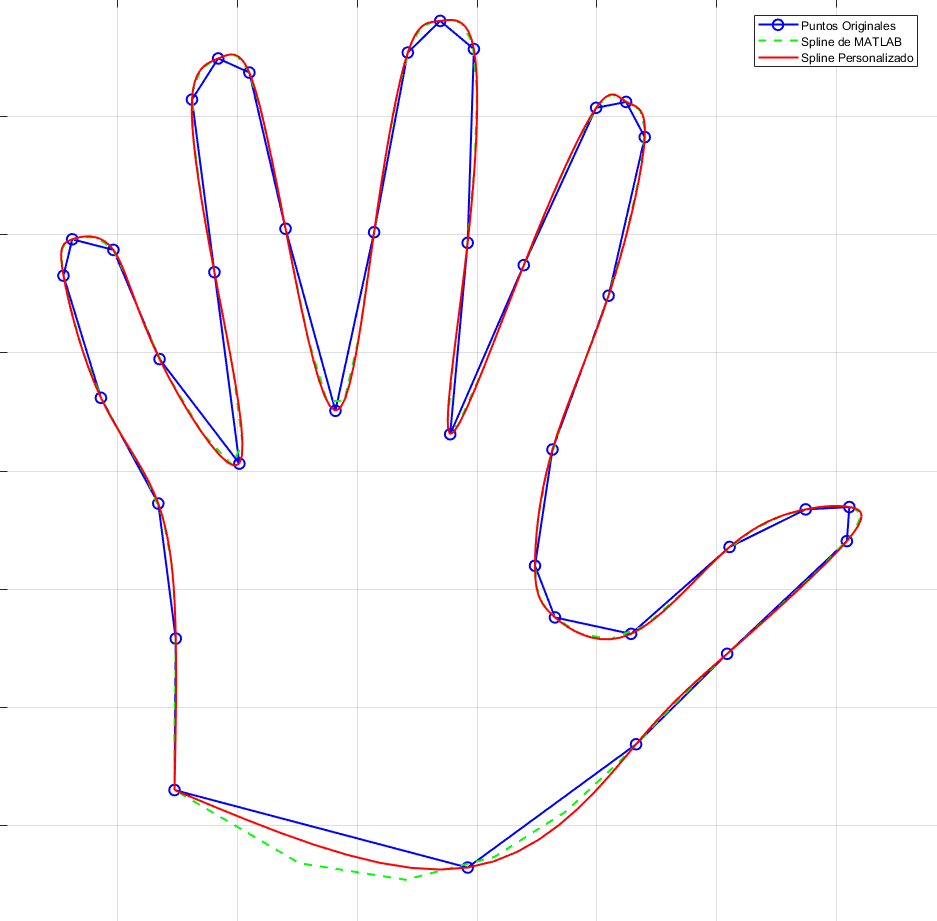
\includegraphics[width=\textwidth]{Figures/mano final.png} % Cambia por el nombre correcto
        \caption{Spline de la mano de Sandra.}
        \label{fig:spline_sandra}
    \end{minipage}
    \hfill
    \begin{minipage}{0.48\textwidth}
        \centering
        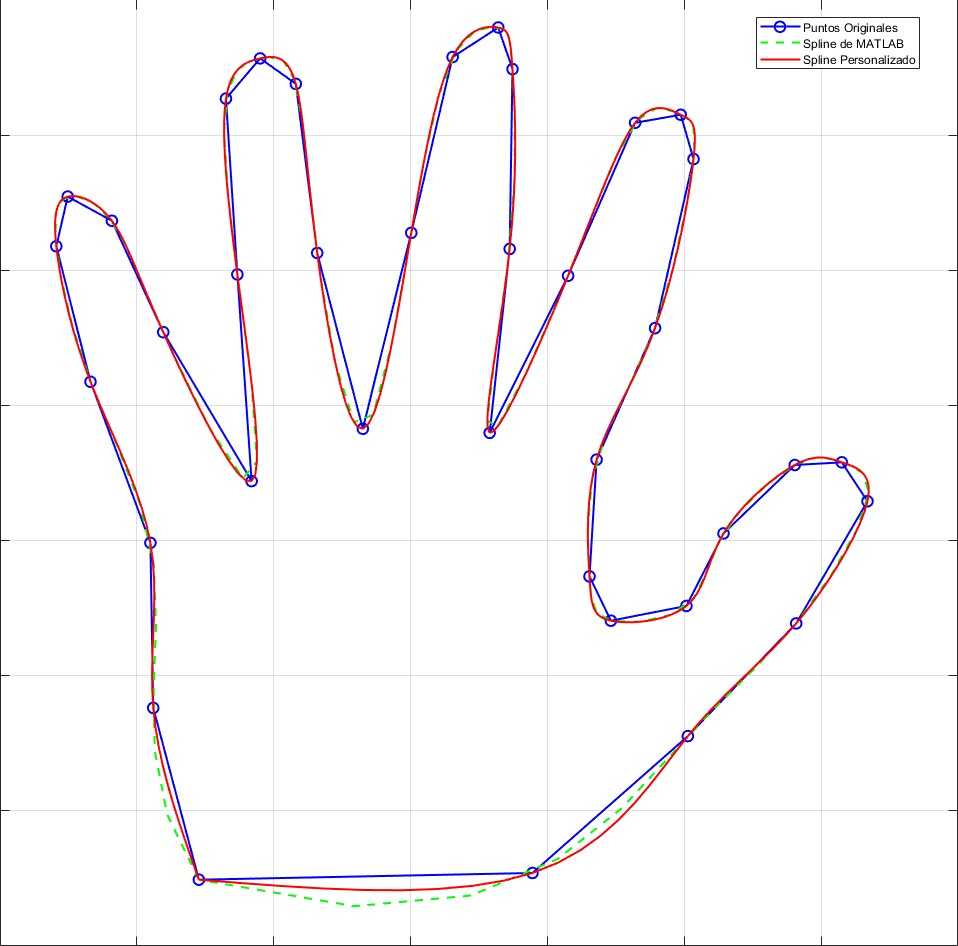
\includegraphics[width=\textwidth]{Figures/mano Andres.jpg} % Cambia por el nombre correcto
        \caption{Spline de la mano de Andrés.}
        \label{fig:spline_andres}
    \end{minipage}
\end{figure}

Los gráficos muestran la interpolación realizada mediante splines cúbicos. En cada imagen, los trazos azules representan los puntos originales, la curva roja corresponde al spline cúbico implementado manualmente y la curva verde representa la interpolación generada por MATLAB.

La interpolación realizada con splines cúbicos genera una aproximación suave y continua a partir de los puntos dados, evitando las oscilaciones bruscas que podrían aparecer con otros métodos, como la interpolación polinómica global. La implementación personalizada resuelve un sistema tridiagonal para obtener las segundas derivadas en los puntos de control, garantizando una transición fluida entre segmentos. Esto se traduce en una curva interpolada que respeta la forma general de los datos originales sin generar artefactos inesperados.  

Al comparar la interpolación con el spline de MATLAB, se pueden notar ligeras diferencias en ciertos tramos. Esto puede deberse a la forma en que cada método maneja las condiciones de frontera y distribuye los puntos interpolados. MATLAB emplea una parametrización interna que puede afectar la forma final de la curva, mientras que la interpolación personalizada usa una parametrización directa basada en la posición secuencial de los puntos. Como resultado, aunque ambas curvas siguen la misma estructura general, hay pequeñas variaciones en la forma en que se suavizan ciertas transiciones. Estas diferencias pueden observarse con mayor claridad en la siguiente figura:  

\begin{figure}[H] % Asegura que la imagen aparezca en la posición deseada
    \centering
    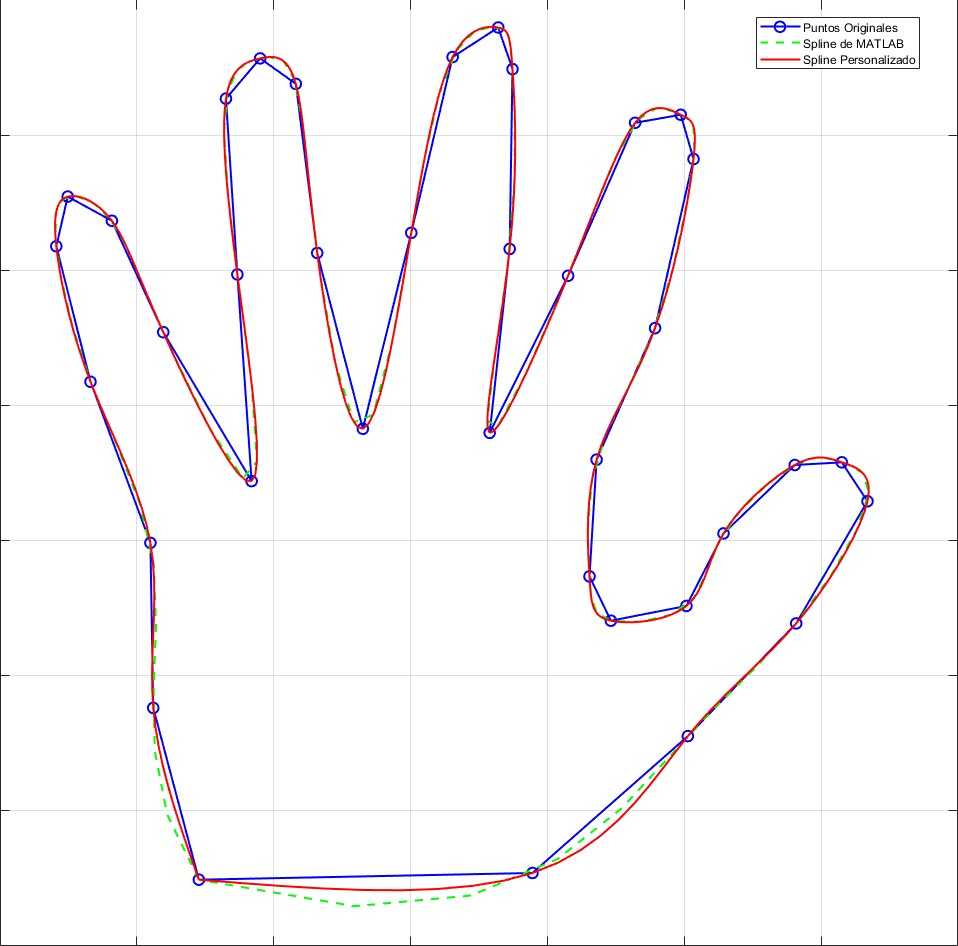
\includegraphics[width=0.5\textwidth]{Figures/mano Andres.jpg} % Cambia el nombre del archivo
    \caption{Vista ampliada de la gráfica en un dedo.}
    \label{fig:detalle_dedo}
\end{figure}  

En términos de exactitud, ambas interpolaciones ofrecen una aproximación adecuada a la forma original. La interpolación manual proporciona una representación fiel y coherente con los datos ingresados, manteniendo una curva suave que se ajusta a la estructura esperada. Aunque hay pequeñas diferencias con MATLAB, estas no implican una pérdida de precisión significativa, sino más bien una variación en la forma en que cada método interpola los segmentos individuales.  

Para visualizar mejor cada interpolación, se presentan las tres gráficas por separado. En estas representaciones individuales, se puede apreciar con mayor claridad cómo se ajusta cada spline a los puntos originales.
\begin{figure}[H]
    \centering
    \begin{minipage}{0.48\textwidth}
        \centering
        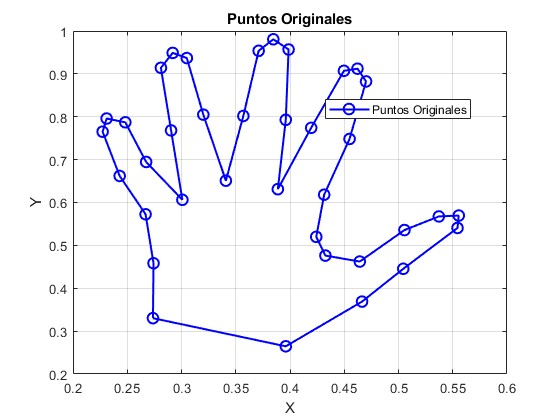
\includegraphics[width=\textwidth]{Figures/puntos originales.jpg} % Cambia por el nombre correcto
        \label{fig:imagen1}
    \end{minipage}
    \hfill
    \begin{minipage}{0.48\textwidth}
        \centering
        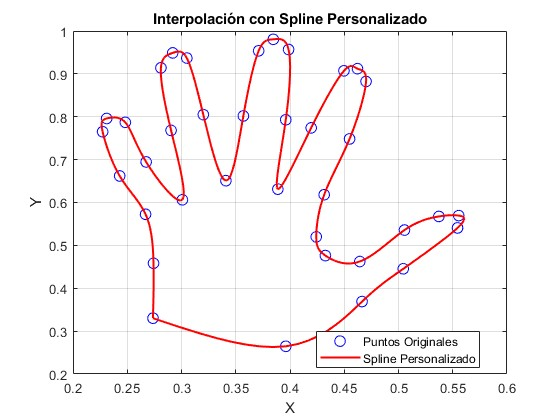
\includegraphics[width=\textwidth]{Figures/interpolacion propia.png} % Cambia por el nombre correcto
        \label{fig:imagen2}
    \end{minipage}

    % Imagen inferior
    \vfill
    \begin{minipage}{0.6\textwidth}
        \centering
        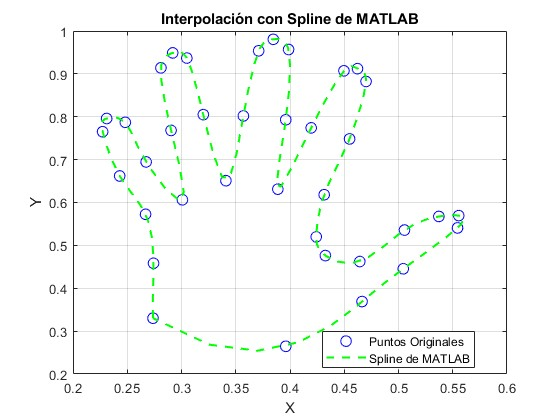
\includegraphics[width=\textwidth]{Figures/interpolacion de matlab.jpg} % Cambia por el nombre correcto
        \label{fig:imagen3}
    \end{minipage}
\end{figure}

  \end{solucion}
\end{homeworkProblem}
 
 \newpage
 \begin{homeworkProblem}
  Sea $f$ analítica sobre un abierto $U$, sea $z_0\in U$ un máximo para $Re(f)$  (parte real de $f$) ($Re(f(z_0)) > Re(f(z)$), para todo $z \in U$). Probar que $f$ es localmente constante en $z_0$.
  \begin{solution}
    Note que $e^{f(z)}$ es analítica en $U$, además $|e^{f(z)}|=e^{Re(f(z))}$, luego la existencia de un máximo para $Re(f)$ implica la existencia de un máximo para $e^{Re(f)}=|e^{f(z)}|$, que por el teorema anterior implicaría que si el máximo es $z_0$, entonces $e^{f(z)}$ es localmente constante en $z_0$ y por ende $f$ es localmente constante en $z_0$.
    \demostrado
  \end{solution}
\end{homeworkProblem}
\begin{homeworkProblem}
  Sea $f$ analítica sobre un abierto $U$, sea $z_0\in U$ un máximo para $Im(f)$  (parte imaginaria de $f$) ($Im(f(z_0)) > Im(f(z)$), para todo $z \in U$). Probar que $f$ es localmente constante en $z_0$.
  \begin{solution}
    Note que $e^{-if(z)}$ es analítica en $U$, además $|e^{-if(z)}|=e^{Im(f(z))}$, luego la existencia de un máximo para $Im(f)$ implica la existencia de un máximo para $e^{Im(f)}=|e^{-if(z)}|$, que por el teorema anterior implicaría que si el máximo es $z_0$, entonces $e^{-if(z)}$ es localmente constante en $z_0$ y por ende $f$ es localmente constante en $z_0$.
    \demostrado
  \end{solution}
\end{homeworkProblem}

 \newpage
 \begin{homeworkProblem}
  Sea $U$ un abierto de $\mathbb{R}^{n}$. Decimos que una función $v\in C^{2}(\overline{U})$ es subarmónica si:
  \begin{align*}
    -\Delta v &\leq 0 &&\text{en $U$.} 
  \end{align*}
  \begin{enumerate}
    \item Demuestre que si $v$ es subarmónica, entonces:
      \begin{align*}
        v(x)&\leq \fint_{B(x,r)}v(y)dy, &&\text{para toda $B(x,r)\subseteq U$.}
      \end{align*}
      \textbf{Sugerencia:} argumente como en la demostración de la propiedad del valor medio para la ecuación de Laplace, es decir, considere $\phi(r)=\fint_{\partial B(x,r)}u(y)dS(y)$ y calcule $\phi'(r)$.
      \begin{solucion}
        Considere $\phi(r)$ tal que si tomamos $B(x,r)\subseteq U$:
        \begin{align*}
          \phi(r)&=\fint_{\partial B(x,r)}v(y)dS(y)\\
          &=\fint_{\partial B(0,1)}v(x+rz)dS(z)
        \end{align*}
        Ahora, si derivamos $\phi$ tenemos que:
        \begin{align*}
          \phi'(r)&=\frac{d}{dr}\fint_{\partial B(0,1)}v(x+rz)dS(z)\\
          &=\fint_{\partial B(0,1)}\nabla v(x+rz)\cdot z dS(z) &&\text{Usando $y=x+rz$.}\\
          &=\fint_{\partial B(0,1)}\nabla v(y)\cdot \frac{y-x}{r}dS(y) &&\text{Como $\frac{y-x}{r}$ es normal a $\partial B(0,1)$.}\\
          &=\frac{1}{|\partial B(0,1)|}\int_{\partial B(0,1)}\nabla v(y)\cdot \eta dS(y)\\
          &=\frac{1}{|\partial B(0,1)|}\int_{\partial B(0,1)}\Delta v(y)dy &&\text{Usando la formula de Green II.}\\
          &\geq 0 &&\text{Ya que $\Delta v(y)\geq0$}
        \end{align*}
        Ahora, como $\phi'(r)\geq 0$, entonces $\phi$ debe de ser una función creciente, por lo que podemos asegurar que:
        \begin{align*}
          \phi(r)&\geq \lim_{r\rightarrow 0} \phi(r)\\
          &\geq \fint_{\partial B(x,r)}v(y)dS(y)\\
          &\geq v(x)
        \end{align*}
        Por lo que podemos asegurar que:
        \begin{align*}
          v(x)&\leq \fint_{\partial B(x,r)}v(y)dS(y)
        \end{align*}
        Ahora, note que:
        \begin{align*}
          \int_{B(x,r)}v(y)dy&\geq \int_{0}^{r}\int_{\partial B(x,s)}v(y)dS(y)ds\\
          &\geq \int_{0}^{r}v(x)|\partial B(x,s)|ds\\
          &\geq v(x)\int_{0}^{r}n\alpha(n)s^{n-1}ds\\
          &\geq v(x)\alpha(n)r^{n}\\
          &\geq v(x)|B(x,r)|
        \end{align*}
        Por lo que podemos concluir en que:
        \begin{align*}
          v(x)&\leq \frac{1}{|B(x,r)|}\int_{B(x,r)}v(y)dy\\
          &\leq \fint_{\partial B(x,r)}v(y)dy
        \end{align*}
        \demostrado
      \end{solucion}
    \item Como consecuencia demuestre que si $U$ es conexo, entonces $\max_{\overline{U}}v=\max_{\partial U}v$.
      \begin{solucion} 
        Suponga que existe $x_0$ tal que $v(x_0)=M=\max_{x\in \overline{U}}v(x)$, entonces suponiendo $0<r_0<d(x_0,\partial U$ y usando el punto anterior se tiene que:
        \begin{align*}
          v(x_0)&\leq\fint_{B(x_0,r_0)}v(y)dy\\
          &\leq M
        \end{align*}
        Ahora, note que $M<M$ es un absurdo, por lo que necesariamente se debe de tener $M=M$, ahora, aprecie que este hecho solo se puede dar si $v(y)=M$ para todo $y\in B(x_0,r_0)$, lo que motiva a pensar en los siguientes subconjuntos de $U$:
        \begin{align*}
          A:=\{x\in U: v(x)=M\}\\
          B:=\{x\in U: v(x)\neq M\}
        \end{align*}
        Note que tanto $A$ como como $B$ son abiertos, ya que para cada $x\in A$ se cumple que existe $B(x,r_x)$ tal que para todo $y\in B(x,r_x)$ se da que $y\in A$, usando el razonamiento que realizamos con $x_0$.\\
        Ahora, note que $B$ también es abierto, ya que dado $x\in B$ ($v(x)\neq M$), tenemos que por la continuidad de $v$ existe un $0<r_x<d(x,\partial U)$ tal que si $y\in B(x,r_x)$, entonces $y\neq M$ y por ende $y\in B$.\\
        Luego, note que $A\cup B=U$ y $A\cap B=\emptyset$, pero como $U$ es conexo, entonces $A=\emptyset$ o $B=\emptyset$, pero como $x_0\in A$, entonces $B=\emptyset$, por lo que podemos afirmar que $v(x)=M$ para todo $x\in U$, además, como $v\in C^{0}(\overline{U})$, entonces $v(x)=M$ para todo $x\in \overline{U}$, por lo que podemos asegurar que:
        \begin{align*}
          \max_{x\in\overline{U}}v(x)=\max_{x\in\partial U}v(x)
        \end{align*}
        \demostrado
      \end{solucion}
    \item Sea $\phi:\mathbb{R}\rightarrow \mathbb{R}$ una función suave convexa ($\phi''>0$). Demuestre que si $u$ es armónica, entonces la función $v=\phi(u)$ es subarmónica.
      \begin{solucion}
        Note que:
        \begin{align*}
          \partial_{x_i}v(x)&=\partial_{x_i}(\phi \circ u)(x)\\
          &=[(\phi'\circ u)(x)][\partial_{x_i}u(x)]\\
          \partial_{x_i^2}v(x)&=[(\phi''\circ u)(x)][\partial_{x_i}u(x)][\partial_{x_i}u(x)]+[(\phi'\circ u)(x)][\partial_{x_i^2}u(x)]\\
          &=[(\phi''\circ u)(x)][\partial_{x_i}u(x)]^2+[(\phi'\circ u)(x)][\partial_{x_i^2}u(x)]
        \end{align*}
        Pero como $\phi''>0$
        \begin{align*}
          \partial_{x_i^2}v(x)&>[(\phi'\circ u)(x)][\partial_{x_i^2}u(x)]
        \end{align*}
        Luego:
        \begin{align*}
          \Delta v(x)&>[(\phi'\circ u)(x)]\Delta u &&\text{Pero como $\Delta u=0$.}\\
          &>0
        \end{align*}
        Por lo que podemos concluir en que $v=\phi(u)$ es subarmónica.
        \demostrado
      \end{solucion}
    \newpage
    \item Demuestre que si $u$ es armónica, entonces $v=|\nabla u|^2$ es subarmónica.
      \begin{solucion}
        Note que, como $u$ es armónica, sus derivadas también lo son, además $\nabla u$ es la suma de sus derivadas e igualmente sabemos que suma de funciones armónicas es armónica, por lo que será suficiente ver que $v=|u|^2$ es armónica para comprobarlo.\\ 
        Suponga $\phi(x)=|x|^2$, utilizando el cálculo del punto anterior y $v=\phi(u)$, es fácil llegar a que:
        \begin{align*}
          \partial_{x_i^2}v(x)&=2[\partial_{x_i}u(x)]^2+[2|u(x)|][\partial_{x_i^2}u(x)]
        \end{align*}
        Por lo que podemos verificar que:
        \begin{align*}
          \Delta v(x)&=2\sum_{i=1}^{n}[\partial_{x_i^2}u(x)]^2+2|u(x)|\Delta u(x)\\
          &=2\sum_{i=1}^n[\partial_{x_i^2}u(x)]^2 &&\text{Ya que $\Delta u(x)=0$.}\\
          &\geq 0
        \end{align*}
        Por lo que podemos concluir que $v$ es subarmónica. 
      \end{solucion}
  \end{enumerate}
\end{homeworkProblem}

 \newpage
 \begin{homeworkProblem}
  Sea $f(z)=\sum_{n=0}^{\infty}a_nz^n$, con radio de convergencia $r$. Probar:
  \begin{itemize}
    \item $g(z)=\sum_{n=1}^{\infty}na_nz^{n-1}$ tiene el mismo radio de convergencia de $f$.
      \begin{solution}
        Sabemos que:
        \begin{align*}
          \lim_{n \to \infty}|a_n|^{\frac{1}{n}}=\frac{1}{r}
        \end{align*}
        luego:
        \begin{align*}
          \lim_{n \to \infty}|na_n|^{\frac{1}{n}}&=\lim_{n \to \infty}|n|^{\frac{1}{n}}|a_n|^{\frac{1}{n}}\\
          &=(1)\left( \frac{1}{r} \right)\\
          &=\frac{1}{r}
        \end{align*}
        de lo que se puede concluir que el radio de convergencia de $g$ es $r$.
        \demostrado
      \end{solution}
    \item $f$ es holomorfa en $D(0,r)$ y $f'(z)=g(z)$.
      \begin{solution}
        Sea $|z|<r$ y $\delta>0$ tal que $|z|+\delta < r$. Sea $h\in\mathbb{C}$ tal que $|h|<\delta$, luego:
        \begin{align*}
          f(z+h)&=\sum_{n=0}^{\infty}a_n(z+h)^{n}\\
          &=\sum_{n=0}^{\infty}a_n(z^n+nz^{n-1}h+h^2p_n(z,h))
        \end{align*}
        donde $p_n(z,h)$ es un polinomio con coeficientes en los enteros.\\
        Note que:
        \begin{align*}
          \left| p_n(z,h) \right|&\leq\left| \sum_{k=2}^{n} \binom{n}{k}\delta^{k-2}z^{n-k}\right|\\
          &\leq \sum_{k=2}^{n}\binom{n}{k}\delta^{k-2}|z|^{n-k}\\
          &\leq p_n(|z|,\delta)
        \end{align*}
        Ahora:
        \begin{align*}
          f(z+h)-f(z)-\sum_{n=1}^{\infty}na_nz^{n-1}h=h^2\sum_{n=2}^{\infty}a_np_n(z,h)
        \end{align*}
        lo que implica:
        \begin{align*}
          \frac{f(z+h)-f(z)}{h}-\sum_{n=1}^{\infty}na_nz^{n-1}&=h\sum_{n=2}^{\infty}a_np_n(z,h)
        \end{align*}
        luego:
        \begin{align*}
          \lim_{h \to 0}\left| h\sum_{n=2}^{\infty}a_np_n(z,h) \right|&\leq \lim_{h \to 0}|h|\left| \sum_{n=2}^{\infty}a_np_n(z,h) \right|\\
          &\leq \lim_{h \to 0}|h|\sum_{n=2}^{\infty}|a_n|p_n(|z|,\delta)\\
          &\leq 0
        \end{align*}
        luego $f$ es diferenciable y su derivada es $g$.
        \demostrado
      \end{solution}
    \item Pruebe $a_n=\frac{f^{(n)}(0)}{n!}$.
      \begin{solution}
        Note que:
        \begin{align*}
          f^{(n)}(z)&=\sum_{k=n}^{\infty}\left(\prod_{i=k-n+1}^{k}i\right)a_k(z)^{k-n}\\
          &=n!a_n+\sum_{k=n+1}^{\infty}\left(\prod_{i=k-n+1}^{k}i\right)a_k(z)^{k-n}
        \end{align*}
        luego $f^{(n)}(0)=n!a_n$, lo que implica $a_n=\frac{f^{(n)}(0)}{n!}$.
        \demostrado
      \end{solution}
    \item Sea $h(z)=\sum_{n=0}^{\infty}\frac{a_n}{n+1}z^{n+1}$. Pruebe que tiene radio de convergencia $r$. (Note que $h'(z)=f(z)$, $h$ se le llama primitiva de $f$).
    \begin{solution}
      Note que:
      \begin{align*}
        \lim_{n \to \infty}\left| \frac{a_{n-1}}{n} \right|^{\frac{1}{n}}&\leq \lim_{n \to \infty}\frac{|a_{n-1}|^{\frac{1}{n}}}{|n|^{\frac{1}{n}}}\\
        &\leq \frac{\lim_{n \to \infty}|a_{n-1}|^{\frac{1}{n}}}{\lim_{n \to \infty}|n|^{\frac{1}{n}}}\\
        &\leq \frac{\frac{1}{r}}{1}\\
        &\leq \frac{1}{r}
      \end{align*}
      luego $h(z)$ tiene radio de convergencia $r$.
      \demostrado
    \end{solution}
  \end{itemize}
\end{homeworkProblem}

 \newpage
 \begin{homeworkProblem}
  Si $f(z)=\sum_{n=1}^{\infty}\frac{z^{2n}}{(2n)!}$. Probar que $f''(z)=f(z)$.
  \begin{solution}
    Usando resultados anteriores:
    \begin{align*}
      f''(z)&=\sum_{n=2}^{\infty}(2n)(2n-1)\frac{z^{2n-2}}{(2n)!}\\
      &=\sum_{n=2}^{\infty}\frac{z^{2n-2}}{(2n-2)!}\\
      &=\sum_{n=1}^{\infty}\frac{z^{2n}}{(2n)!}\\
      &=f(z)
    \end{align*}
  \end{solution}
\end{homeworkProblem}
\begin{homeworkProblem}
  Si $f(z)=\sum_{n=0}^{\infty}\frac{z^{2n}}{(n!)^2}$. Probar que $z^2f''(z)+zf'(z)=4z^2f(z)$.
  \begin{solution}
    Calculemos $f'$ y $f''$:
    \begin{align*}
      f'(z)&=\sum_{n=1}^{\infty}(2n)\frac{z^{2n-1}}{(n!)^2}\\
      f''(z)&=\sum_{n=1}^{\infty}(2n)(2n-1)\frac{z^{2n-2}}{(n!)^2}
    \end{align*}
    luego:
    \begin{align*}
      z^2f''(z)+zf'(z)&=\sum_{n=1}^{\infty}(2n)\frac{z^{2n}}{(n!)^2}+\sum_{n=1}^{\infty}(2n)(2n-1)\frac{z^{2n}}{(n!)^2}\\
      &=\sum_{n=1}^{\infty}4n^2\frac{z^{2n}}{(n!)^2}\\
      &=4z^2\sum_{n=1}^{\infty}\frac{z^2n-2}{((n-1)!)^2}\\
      &=4z^2\sum_{n=0}^{\infty}\frac{z^{2n}}{(n!)^2}\\
      &=4z^2f(z)
    \end{align*}
  \end{solution}
\end{homeworkProblem}

 \newpage
 \begin{homeworkProblem}
  Calcular $(-3+4i)^{-\frac{3}{2}}$.
  \begin{solution}
    Por el punto anterior sabemos que:
    \begin{align*}
      (-3+4i)^{\frac{3}{2}}=5\sqrt{5}e^{i\frac{3arctan\left( \frac{4}{-3} \right)+2k\pi}{2}}
    \end{align*}
    De lo que se puede concluir que:
    \begin{align*}
      (-3+4i)^{-\frac{3}{2}}=\frac{e^{-i\frac{3arctan\left( \frac{4}{-3} \right)+2k\pi}{2}}}{5\sqrt{5}}
    \end{align*}
  \end{solution}
\end{homeworkProblem}

 \newpage
 \begin{homeworkProblem}
  Si$J(z) = \sum_0^\infty \frac{(-1)^n}{(n!)^2} \left(\frac{z}{2}\right)^{2n}$. Probar $z^2 J''(z) + zJ'(z) + z^2 J(z) = 0$.
  \begin{solution}
    Calculemos $zJ'$ y $z^2J''$ 
    \begin{align*}
      zJ'(z) &= \sum_{n=1}^{\infty} \frac{(-1)^n}{(n!)^2} \frac{(2n)}{2^{2n}} z^{2n}\\
      z^{2}J''(z) &= \sum_{n=1}^{\infty} \frac{(-1)^n}{(n!)^2} \frac{(2n)(2n-1)}{2^{2n}} z^{2n}
    \end{align*}
    Ahora sumemos:
    \begin{align*}
      z^2J''(z)+zJ'(z)&=\sum_{n=1}^{\infty} \frac{(-1)^n}{(n!)^2} \frac{(2n)(2n)}{2^{2n}} z^{2n}\\
      &=-\sum_{n=0}^{\infty} \frac{(-1)^n4(n+1)^2}{2^{2n+2}((n+1)!)^2} z^{2n+2}\\
      &=-\sum_{n=0}^{\infty} \frac{(-1)^n}{(n!)^2}z^2\left( \frac{z}{2} \right)^{2n} = -z^2J(z)
    \end{align*}
  \end{solution}
\end{homeworkProblem}

 \newpage
 \begin{homeworkProblem}
  Para $k$ entero positivo, sea $J_k(z) = \sum_{0}^{\infty} \frac{(-1)^n}{n! (n+k)!} \left( \frac{z}{2} \right)^{2n+k}$. Probar:
  \begin{align*}
    z^2 J_k''(z) + zJ_k'(z) + (z^2 - k^2) J_k(z) = 0.   
  \end{align*}
  \begin{solution}
    Dada la función:
    \begin{align*}
      J_k(z) &= \sum_{n=0}^{\infty} \frac{(-1)^n}{n! (n+k)!} \left( \frac{z}{2} \right)^{2n+k},
    \end{align*}
    calculamos sus derivadas y productos:
    \begin{align*}
      zJ_k'(z) &= \sum_{n=0}^{\infty} \frac{(-1)^n}{n! (n+k)!} (2n+k)\left( \frac{z}{2} \right)^{2n+k} \\
      z^2J_k''(z) &= \sum_{n=0}^{\infty} \frac{(-1)^n}{n! (n+k)!} \cdot (2n+k)(2n+k-1) \left( \frac{z}{2} \right)^{2n+k}.
    \end{align*}
    Sustituyendo en la ecuación:
    \begin{align*}
      z^2 J_k''(z) + z J_k'(z) + (z^2 - k^2) J_k(z),
    \end{align*}
    obtenemos:
  \end{solution}
\end{homeworkProblem}

%%%%%%%%%%%%%%%%%%%%%%%%%%%%%%%%%%%%%%%%%%%%%%%%%%%%%%%
\end{document}

